\setcounter{secnumdepth}{1}

\section{Einführung}

Javascript ist im Aufwind mehr denn je. Sie ist die meist genutzte Programmiersprache unter Entwicklern. Laut der diesjährigen Umfrage von Stackoverflow belegte sie zum sechsten mal in Folge den ersten Platz.\cite{programming-language-survey} Doch woher kommt dieser Erfolg? \\
Wenn es um das Web geht, war Javascript als Skriptsprache schon immer Vorreiter. Doch diese Sprache hat seine Stärken auch in der Vielfalt seiner Einsatzmöglichkeiten. Wie mit dem Framework Node.js, dass ab 2009 in Erscheinung getreten ist, war es Möglich Server-seitigen Javascript-Code zu implementieren. Dies hatte zur Folge, dass man sich nicht mit multiplen Programmiersprachen auseinandersetzen musste. Man hatte eine Vereinheitlichung in seiner Code-Basis gefunden. Zudem bietet Node.js mit npm als Paketmanager die größte Auswahl an Open-Source-Libraries. Ein weiterer Punkt ist die Multi-Plattform-Kompatibilität die Javascript z.B. mit dem Framework Angular offenbart. Mit diesen Framework ist es Möglich mit einer Code-Basis sowohl Web-Anwendungen als auch Apps für mobile Geräte zu entwickeln. Da Javascript's Kompilierung vom Betriebssystem unabhängig ist, ist der Übergang von der Webentwicklung zur mobilen Entwicklung reibungslos. Und genau das bietet auch Typescript. Da Typescript ein sog. \textbf{Superset} von Javascript ist, kann jeder Code von Javascript auch in Typescript interpretiert werden. Der Unterschied zu Typescript und Javascript liegt in ihrer statischen Typisierung. Das bedeutet, dass Variablen, Methoden und Funktionsparameter im Vorfeld mit einem Typ versehen werden. Aufgrund dessen können Bugs zur Laufzeit schneller erkannt werden. Zudem lässt sich diese Sprache leicht modular aufbauen. Dadurch können Entwicklerteams in Unternehmensprojekte die Code-Struktur besser organisieren und dokumentieren.\\\\

\noindent
Doch mit der Vielfalt steigt auch die Komplexität der Sprache. Schon zum vierten Jahr in Folge erschien eine neue Version von Javascript, die neueste Features mit sich bringt. Beispielsweise ermöglichen Promises und async await einen neuen Ansatz zur asynchronen Verarbeitung. Somit werden Applikation, die ereignisgesteuert operieren, neue Möglichkeiten geboten. Mit Callbacks, Promises und Streams bekommen Entwickler verschiedene Optionen der asynchronen Datenverarbeitung zur Verfügung. Die Einsatzmöglichkeiten in einem Projekt können variieren, jedoch welcher Ansatz in welcher Situation sinnvoller erscheint, ist besonders für Entwickler mit wenig Erfahrung schwer zu erkennen.

\subsection{Zielsetzung}

Ziel der Arbeit ist die Betrachtung und Aufbereitung des Einsatzes von Sprachmitteln zur asynchronen Verarbeitung in Typescript in einer Form, die Einsteigern in die Thematik hilft, die unterschiedlichen Konzepte voneinander abzugrenzen und richtig einzusetzen. Dazu soll asynchrone Verarbeitung insgesamt anhand brauchbarer und für den Einsatz von Typescript typischer Szenarien motiviert werden. Es werden die zur Verfügung stehenden Sprachmittel wie Callbacks, Promises und Observables mit ihren jeweiligen Features vorgestellt. Nach dem Lesen dieser Arbeit soll der Leser ein gewisses Verständnis dafür gewonnen haben, welche der vorgestellten Sprachmitteln für welchen Anwendungsfall besser geeignet ist.\\\\

\noindent
Zielgruppe dieser Arbeit sind Personen, die Grundkenntnisse in der Sprache Javascript/Typescript vorweisen können. Des Weiteren sollte man von dem Modell der asynchronen Datenverarbeitung wie Callbacks, Promises und Oberservables schon mal gehört haben, da diese in der Arbeit gegenübergestellt werden.

\subsection{Aufbau}

In dieser Arbeit werden die jeweiligen Ausarbeitungen der Ansätze mit Code-Beispielen unterstützt. Neben simulierten Anwendungsbeispielen zum Einstieg werden auch praxisnahe Beispiele wie z.B. einen Aufruf an einer API-Endstelle dargestellt. Das Projekt lässt sich in den Modulen Callbacks, Promises, Async-Await und RxJS unterteilen. Diese drei Module haben jeweils eine introduction.ts Datei zur Einführung, eine stories.ts Datei, die entweder Funktionen oder Klassen anbietet und eine stories-usage.ts Datei, die diese Klassen oder Funktionen ausführt. Das Repository für die Code-Projekt ist zu finden unter: 

\begin{center}
\url{https://github.com/MarcoLeko/async-patterns.git}
\end{center}

\noindent
Zu beachten ist, dass vor dem Ausführen des Projektes \textbf{Node.js} auf dem Rechner installiert sein muss, um den integrierten Paket-Manager \textbf{npm} nutzen zu können. Da \textbf{RxJS} nicht von vornherein von Javascript mitgeliefert wird, wird eine sog. \glqq Third-Party Library\grqq{} dafür benötigt. Sobald npm installiert ist, muss in dem Stammverzeichnis des Projekts \textbf{npm install} ausgeführt werden, um die jeweiligen Abhängigkeiten dieser Libraries herunterzuladen. Node.js kann man unter folgendem Link herunterladen:

\begin{center}
\url{https://nodejs.org/en/}
\end{center}

\section{Grundlagen}

\subsection{Typescript}
Typescript. Bereits der Name sagt schon was diese Sprache ausmacht. Sie ist eine typisierte Form der Skriptsprache Javascript. Besonders Javascript-Entwickler sträubten sich Anfangs mit der Sprache auseinanderzusetzen. Die Stärke von Javascript liegt in ihrer Flexibilität und der Tatsache nicht mehr code schreiben zu müssen als man braucht. Doch den Kompromiss den man mit Typescript eingeht, zahlt sich am Ende mit dem Zuwachs der Projektgröße aus. Da der Typescript Kompiler bereits Fehler beim Kompilieren erkennt, stellt sich die Frage, ob man lieber Fehler beim Entwickeln oder in der Produktion eines Projekts entdecken möchte. Dabei ist das \textbf{Tooling} der größte Vorteil von Typescript. Wenn man mit Typ-Annotationen oder mit Libraries, die streng typisiert sind, arbeitet, wird der Code von der Entwicklungsumgebung automatisch dokumentiert. Das heißt beim Entwickeln mit einem Code-Editor wird nicht zusätzlich verlangt, die Dokumentation der benötigten Library zu öffnen, um jede einzelne Methode zu sehen. Wenn man nun von einem reinen Javascript-Hintergrund kommt, gibt es so gut wie keine Lernkurve die Sprache zu bewältigen. Das liegt daran, dass jeder valide Code von Javascript auch in Typescript ausführbar ist. Der Lernprozess steigt mit zunehmender Nutzung.

\subsubsection{Beispiel}

\begin{figure}[H]
\begin{lstlisting}[basicstyle=\small]
class Greeter {
    greeting: string;
    constructor (message: string) {
        this.greeting = message;
    }
    greet() {
        return "Hello, " + this.greeting;
    }
}  
\end{lstlisting}
\caption{Typescript Klasse \cite{typescript-example}}
\end{figure}

\begin{figure}[H]
\begin{lstlisting}[basicstyle=\small]
var Greeter = (function () {
    function Greeter(message) {
        this.greeting = message;
    }
    Greeter.prototype.greet = function () {
        return "Hello, " + this.greeting;
    };
    return Greeter;
})(); 
\end{lstlisting}
\caption{Überführung in Javascript \cite{typescript-example}}
\end{figure}

\noindent
Typescript selbst kann nicht selbständig ausgeführt werden. Das heißt in einem Browser oder auf einem Server wird unter Umständen immer noch Javascript genutzt. Mit dem Typescript Compiler werden daher Dateien mit dem Suffix *.ts in *.js überführt. Im oberen Code-Schnipsel wurden die variablen und die Klassenmethoden nach Typescript-Standard deklariert. Diese Typen werden beim transpilieren in Javascript ignoriert. Der Kompiler prüft dann, ob beim übergeben eines Parameters in den Konstruktor ein string Wert eingesetzt wird. Wenn nicht, wird dies als ein Fehler erkannt. In der vom Kompiler auf Javascript übersetzten Version werden die erstellten Klassen und Typen vollständig eliminiert. Was verbleibt ist die Übersetzung der Methode greet() und des Konstruktors. Zudem werden auch nicht direkt deklarierte (implizite) Typen übersetzt. Wie in diesem Fall wird erkannt, dass die Methode greet() einen String-Wert zurückgibt. Ungleich wie mit Java oder C\# gewährleistet Typescript aus der streng typisierten Welt rauszufahren.

\begin{figure}[H]
\begin{lstlisting}[basicstyle=\small]
let count: any = 23;

count = 'Oops transformed to string!'
\end{lstlisting}
\end{figure}

\noindent
Der Kompiler würde hierbei keinen Fehler anzeigen. Obwohl im Idealfall auf die \textbf{any} Notation verzichtet werden sollte, wird dennoch Javascripts Flexibilität geboten. 

\subsubsection{Kompiler}
Ein großer Vorteil von Typescript ist die Möglichkeit auf verschiedene Javascript/Ecmascript Version zu transpilieren. Wenn bestimmte Browser Javascripts neuster Feature noch nicht unterstützen, kann das Kompilat auf ältere Ecmascript Versionen übersetzt werden. Diese Konfiguration wird mit Hilfe einer \textbf{tsconfig.json} Datei bewältigt. Die Auflistung einer solchen Datei zeigt, dass es sich hierbei um das Stammverzeichnis des Projekts handelt. Hier können die Kompiler-Optionen für Typescript gesetzt werden oder Dateien von der Übersetzung ein- oder ausgeschlossen werden. Ein Beispiel für die Konfiguration einer solchen Datei könnte wie folgt aussehen: 

\begin{figure}[H]
\begin{lstlisting}[basicstyle=\small]
{
  "compilerOptions": {
    "target": "esnext",
    "module": "commonjs",
    "declaration": false,
    "sourceMap": true,
    "noImplicitAny": false,
    "typeRoots": [
      "node_modules/@types"
    ],
    "downlevelIteration": true
  },
  "include": [
    "src/**/*"
  ]
} 
\end{lstlisting}
\caption{Auflistung einer tsconfig.json Datei}
\end{figure}

\noindent
Hier kann z.B. mit der Regel \glqq noImplicitAny\grqq{} festgelegt werden, dass Methoden als auch Parameter und Variablen getypt werden müssen bei ihrer Deklaration. Sind sie nicht getypt: Bedeutet dies für den Kompiler sie sind als any deklariert. Dies würde zu einem Kompilefehler führen.\cite{tsconfig} Mit dem Wert \glqq target\grqq{} wird die zu nutzende Javascript Version eingestellt. Wenn der Wert nicht bestimmt ist, wird standardmäßig nach es3 übersetzt. Um stets die aktuellste Version zu nutzen, wird in diesem Fall wird \textbf{esnext} angegeben.\\

\noindent
Zu beachten ist, dass die Konfiguration dieser Datei nur Fehler beim erstellen eines Kompilats entdeckt. Fehler zur Laufzeit sind von der Konfiguration ausgeschlossen. Zudem wird in jedem Fall eine Javascript Datei erstellt, auch wenn der Kompiler einen Fehler anzeigt. Diese Datei ist potenziell auch lauffähig. Um Typescript zu Kompilieren muss im Terminal unter dem Verzeichnis einer Typescript-Datei \textbf{tsc} eingegeben werden. In den für diese Arbeit genutzten Code-Beispiele werden die Startskripte von npm ausgeführt. Ein Skriptbefehl kann wie folgt aussehen:

\begin{figure}[H]
\begin{lstlisting}[basicstyle=\small]
  ...
  "scripts": {
    "start": "webpack --watch",
    "build": "webpack"
  }, 
\end{lstlisting}
\caption{Auflistung ist unter der \textbf{package.json} Datei zu finden}
\end{figure}

\noindent
Wie man hier sehen kann führt \textbf{npm run start} nicht tsc aus, sondern \textbf{webpack --watch} aus. Webpack ist ein sog. \textbf{Module-Loader}. Mit ihm ist es Möglich Klassen/Interfaces/Funktionen zu im- und exportieren. Da Third-Party Libraries in der Applikation genutzt werden, die externe Klassen und Funktionen mitliefern, ist die Nutzung von Module-Loaders unabdingbar. Zudem wird mit Hilfe von Webpack Typescript-Dateien (je nach Konfiguration), inklusive aller involvierten Importe und Exporte, zu einer zentralen Javascript-Datei gebündelt. In der Webpack Konfiguration muss lediglich eine Eingangsdatei definiert werden. Mit der Einstellung --watch werden Veränderung des Codes in Echtzeit kompiliert. Sollten nun Änderungen im Code vorgenommen werden, erstellt Webpack ein neues Bündel. Nach dem Kompilieren muss nur noch die HTML-Seite geöffnet werden. Um mehr von Typescript und z.B. dessen Nutzung mit Module-Loaders zu erfahren, sollte die offizielle Dokumentation von Microsoft durchgegangen werden.

\begin{center}
\url{https://www.typescriptlang.org/docs/home.html} 
\end{center}

\subsection{Terminologie}

Um die Abgrenzung von verschiedenen asynchronen Sprachmitteln zu beherrschen, muss vorerst geklärt werden, was Asynchronität bedeutet.\\\\

\noindent
Der zentrale Teil eines Computers, welches Programme und einzelne Schritte zum Ausführen bringt, ist der Prozessor. Die Geschwindigkeit in der eine Schleife von einem Programm ausgeführt wird, hängt von der Geschwindigkeit des Prozessors ab. Programme interagieren jedoch mit Operationen außerhalb des Zuständigkeitsbereiches eines Prozessors, wie z.B. die Kommunikation über ein Netzwerk oder Abfragen von Daten von der Festplatte. Solche Operationen hängen von anderen Ressourcen ab und brauchen Zeit. In solchen Szenarien wäre es unvorteilhaft, wenn der Prozessor, anstatt andere Operationen in der Zwischenzeit auszuführen, im Leerlauf stecken würde. Genau für solche Aufgaben ist das Betriebssystem da. Das Betriebssystem sorgt dafür, dass Kapazitäten des Prozessors auf parallel laufende Programme wechselt, während es auf die Antwort von ausgeführten Operationen wartet. Es entstehen dabei verschiedene \glqq Threads\grqq{}. Und hier kommt die Asynchronität ins Spiel:

\subsubsection{Asynchronität}

Ein \textbf{asynchrones} Programmiermodell erlaubt multiple Abläufe zum selben Zeitpunkt. Wenn eine Aktion ausgeführt wird, läuft das Programm in einem anderen \glqq Thread\grqq{} weiter. Sollte die Operation fertig gestellt sein, wird das Programm informiert und liefert das Ergebnis zurück. Ein Beispiel dafür wäre das Suchen von Dateien auf einer Festplatte.\cite{asynchronitaet}

\subsubsection{Synchronität}

In einem \textbf{synchronen} Programmiermodell entstehen Abläufe sequenziell. Wenn eine Funktion mit einer zeitintensiven Aktion abgerufen wird, wird das Ergebnis erst nach dem Beenden der Operation zurückgegeben. In diesem Zeitintervall werden keine Nebenoperationen ausgeführt.\cite{asynchronitaet}\\

\noindent
Man kann ein synchrones und asynchrones Modell mit einem kleinem Beispiel vergleichen: Eine Anwendung die zwei Ressourcen aus einem Netzwerk anfragt und die Ergebnisse miteinander kombiniert. In einer synchronen Umgebung würde man dies mit einem Funktionsaufruf nach dem anderen bewältigen. Das hat den Nachteil, dass die zweite Funktion erst dann ausführt, wenn die erste fertig ist. Die Gesamtzeit der Ausführung ist die Summe der Antwortzeiten der beiden Anfragen. Die Lösung dafür ist ein synchrones Programmverhalten mit mehreren kontrollierten Threads. Ein Thread ist ein Ausführungsstrang, der seine eigene Zeitleiste besitzt und innerhalb dieser Operationen ausführt. Ein zweiter Thread könnte zum selben Zeitpunkt die Funktion aufrufen und wenn beide Threads das Ergebnis geliefert bekommen resynchronisieren sie sich und kombinieren ihre Ergebnisse. Im folgenden Diagramm repräsentieren die blauen Linien die Zeit, in der das Programm ausführt und die roten Linien repräsentieren die Zeit, in der auf die Antwort gewartet wird.\cite{asynchronitaet}

\begin{center}
\begin{figure}[H]
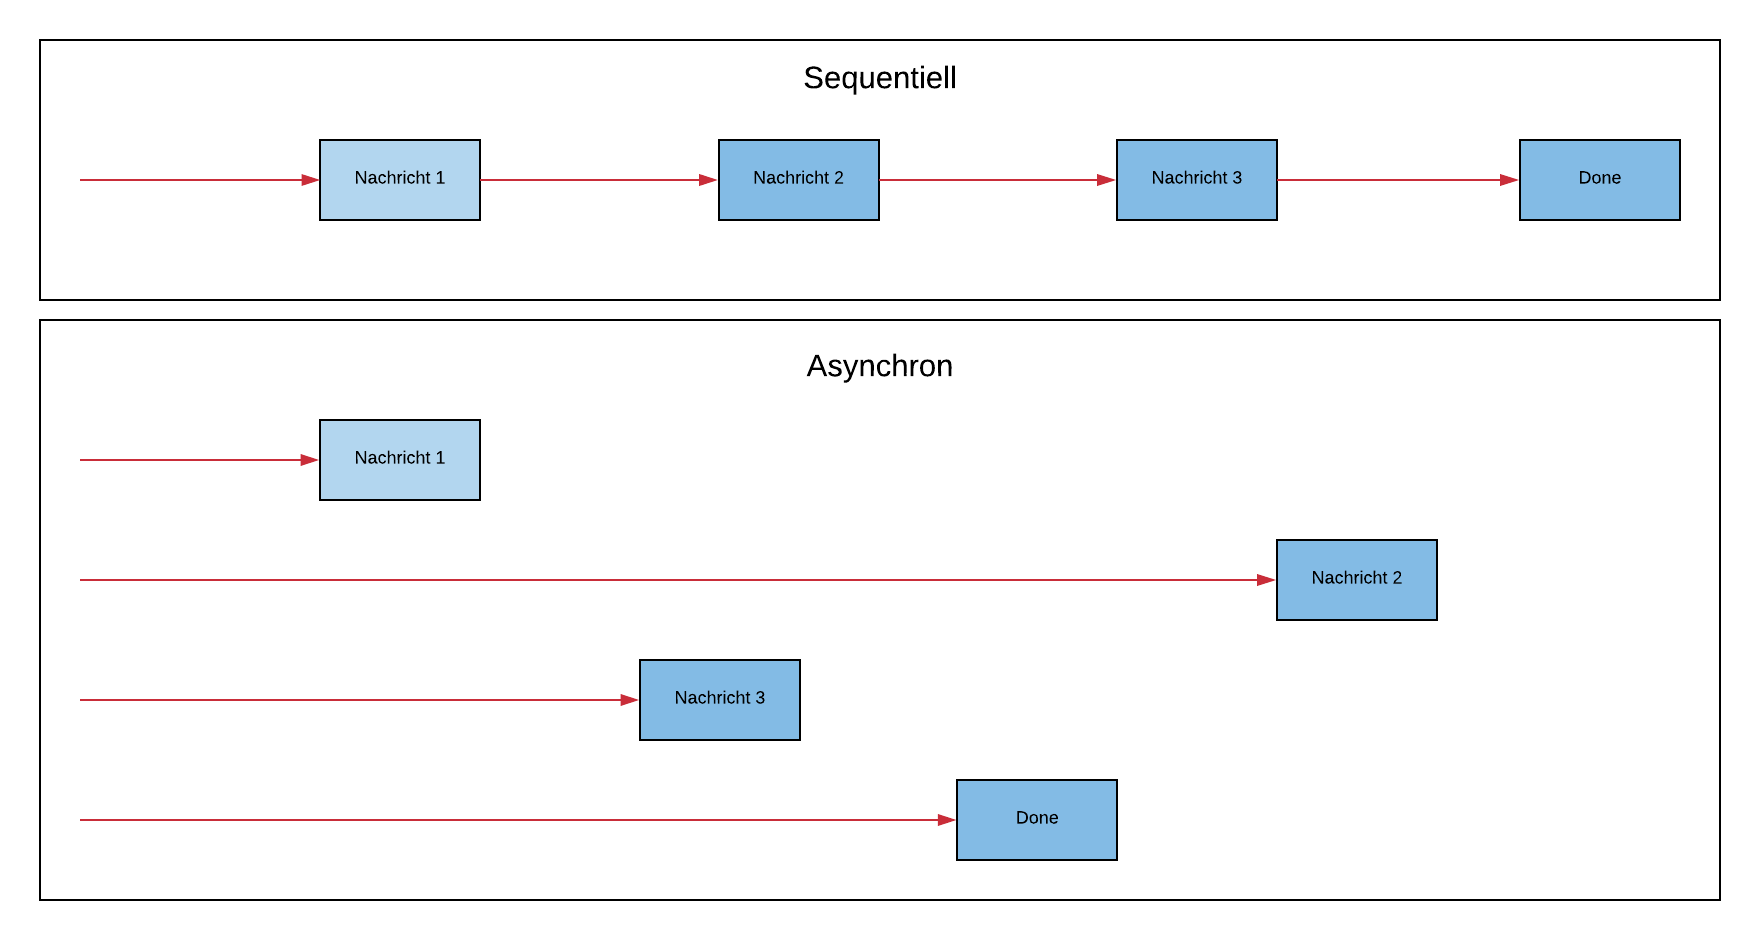
\includegraphics[width=12cm]{synchron-vs-asynchron-diagram}
\end{figure}
\end{center}

\noindent
Im synchronen Modell ist die Zeit der Netzwerkanfrage ein Teil der Zeitleiste. Im asynchronen Modell hingegen führt das Starten einer asynchronen Operation zu einer neuen Zeitleiste. Zusammenfassend kann man also sagen, dass in dem synchronen Modell implizit auf die Aktionen gewartet wird, und in dem asynchronen Modell explizit.